\documentclass{article}
\usepackage{graphicx} % Required for inserting images

\title{ECN 310}
\author{ltsippel }
\date{November 2023}

% set margins and spacing
\addtolength{\textwidth}{1.3in}
\addtolength{\oddsidemargin}{-.65in} %left margin
\addtolength{\evensidemargin}{-.65in}
\setlength{\textheight}{9in}
\setlength{\topmargin}{-.5in}
\setlength{\headheight}{0.0in}
\setlength{\footskip}{.375in}
\renewcommand{\baselinestretch}{1.0}
\linespread{1.0}

% load miscellaneous packages
\usepackage{csquotes}
\usepackage[american]{babel}
\usepackage[usenames,dvipsnames]{color}
\usepackage{graphicx,amsbsy,amssymb, amsmath, amsthm, MnSymbol,bbding,times, verbatim,bm,pifont,pdfsync,setspace,natbib}

% enable hyperlinks and table of contents
\usepackage[pdftex,
bookmarks=true,
bookmarksnumbered=false,
pdfview=fitH,
bookmarksopen=true,hyperfootnotes=false]{hyperref}

% define environments
\newtheorem{definition}{Definition}
\newtheorem{fact}{Fact}
\newtheorem{result}{Result}
\newtheorem{proposition}{Proposition}



\begin{document}
\title{Dementia in the Elderly and Education}
\author{Ixora Artis\thanks{Syracuse University, Economics Department. Email: kbuzard@syr.edu.} \and Sophie Haber\thanks{abc} \and Abigail Mondin\thanks{abc} \and Luke Sippel}
\date{\vskip-.1in \today}
\maketitle

\vskip.3in
\begin{center} {\bf Abstract} \end{center}
\begin{quote}
{\small Insert abstract text here: 75-200 word, very high-level summary of your project.}
\end{quote}

\bigskip
\section{Introduction} \label{sec:introduction}

Answer the questions
\begin{enumerate}
    \item Why should the reader care?
    \item Why did you choose this topic?
    \item What question will you answer? How will you do it?
    \item What did you find?
    \item Give a "road map" of the paper. Where will the reader find the various parts of your work?
   \begin{itemize}
       \item In Section~\ref{sec:literature}, we review the literature. 
       \item In Section~\ref{sec:data} , we describe our data.
       \item In Section~\ref{sec:result} , we explain what analyses we did and provide evidence to explain what our results mean. 
       \item In Section~\ref{sec:discussion} , we explore the implications of our results. 
       \item And in Section~\ref{sec:conclusion} ,  reestablish our findings, communicate how our data might have effected our results, and talk about our big picture goal. 
   \end{itemize}
\end{enumerate}

\section{Literature Review} \label{sec:literature}

Discuss at least five papers that are closely related to your results (more is better). Explain how they're related. Did you find something similar, or different? Did you look at a different context? Different time period? Different level of detail?

\section{Data}
\label{sec:data}


In our data we have a breakdown of different education levels. 

-----------------------------------------
                             |  Frequency
-----------------------------+-----------
r highest level of education |           
  0                          |         19
  1                          |         10
  2                          |         13
  3                          |         21
  4                          |         16
  5                          |         16
  6                          |         94
  7                          |         20
  8                          |         75
  9                          |        107
  10                         |        139
  11                         |        206
  12                         |      1,252
  13                         |        449
  14                         |        602
  15                         |        203
  16                         |        749
  17                         |        505
  97                         |         53
  98                         |         16
  99                         |          2
  Total                      |      4,567
-----------------------------------------

------------------------
            |  Frequency
------------+-----------
rate memory |           
  1         |      1,297
  2         |      4,753
  3         |      8,121
  4         |      4,816
  5         |        965
  8         |         16
  9         |          2
  Total     |     19,970
------------------------

\begin{table}
    \centering
    \begin{tabular}{cc}
         Rate Memory& Frequency\\
         Excellent& 1,297\\
         Very Good& 4,753\\
         Good& 8,121\\
         Fair& 4,816\\
         Poor& 965\\
         Don't Know& 16\\
         Refused& 2\\
         Total& 19,970\\
    \end{tabular}
    \caption{Caption}
    \label{tab:my_label}
\end{table}


-----------------------------------------
                             |  Frequency
-----------------------------+-----------
compare mem to prev wave- pc |           
  1                          |          6
  2                          |        163
  3                          |         48
  9                          |          1
  Total                      |        218
-----------------------------------------

\begin{figure}
    \centering
    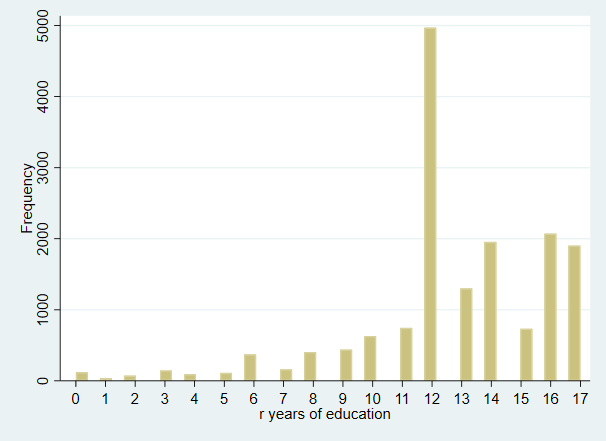
\includegraphics[width=0.5\linewidth]{frequency_histogram_pz216.png}
    \caption{Enter Caption}
    \label{fig:enter-label}
\end{figure}


Describe your data. Where you got it from, how it was generated, what variables you'll use, what data cleaning steps you had to take, where your processed data, code and documentation is stored.

In a published paper, a lot of this detail will be in a data appendix. For the purposes of this report, include it all here (this may be the longest section of your report).!

\begin{figure}
    \centering
    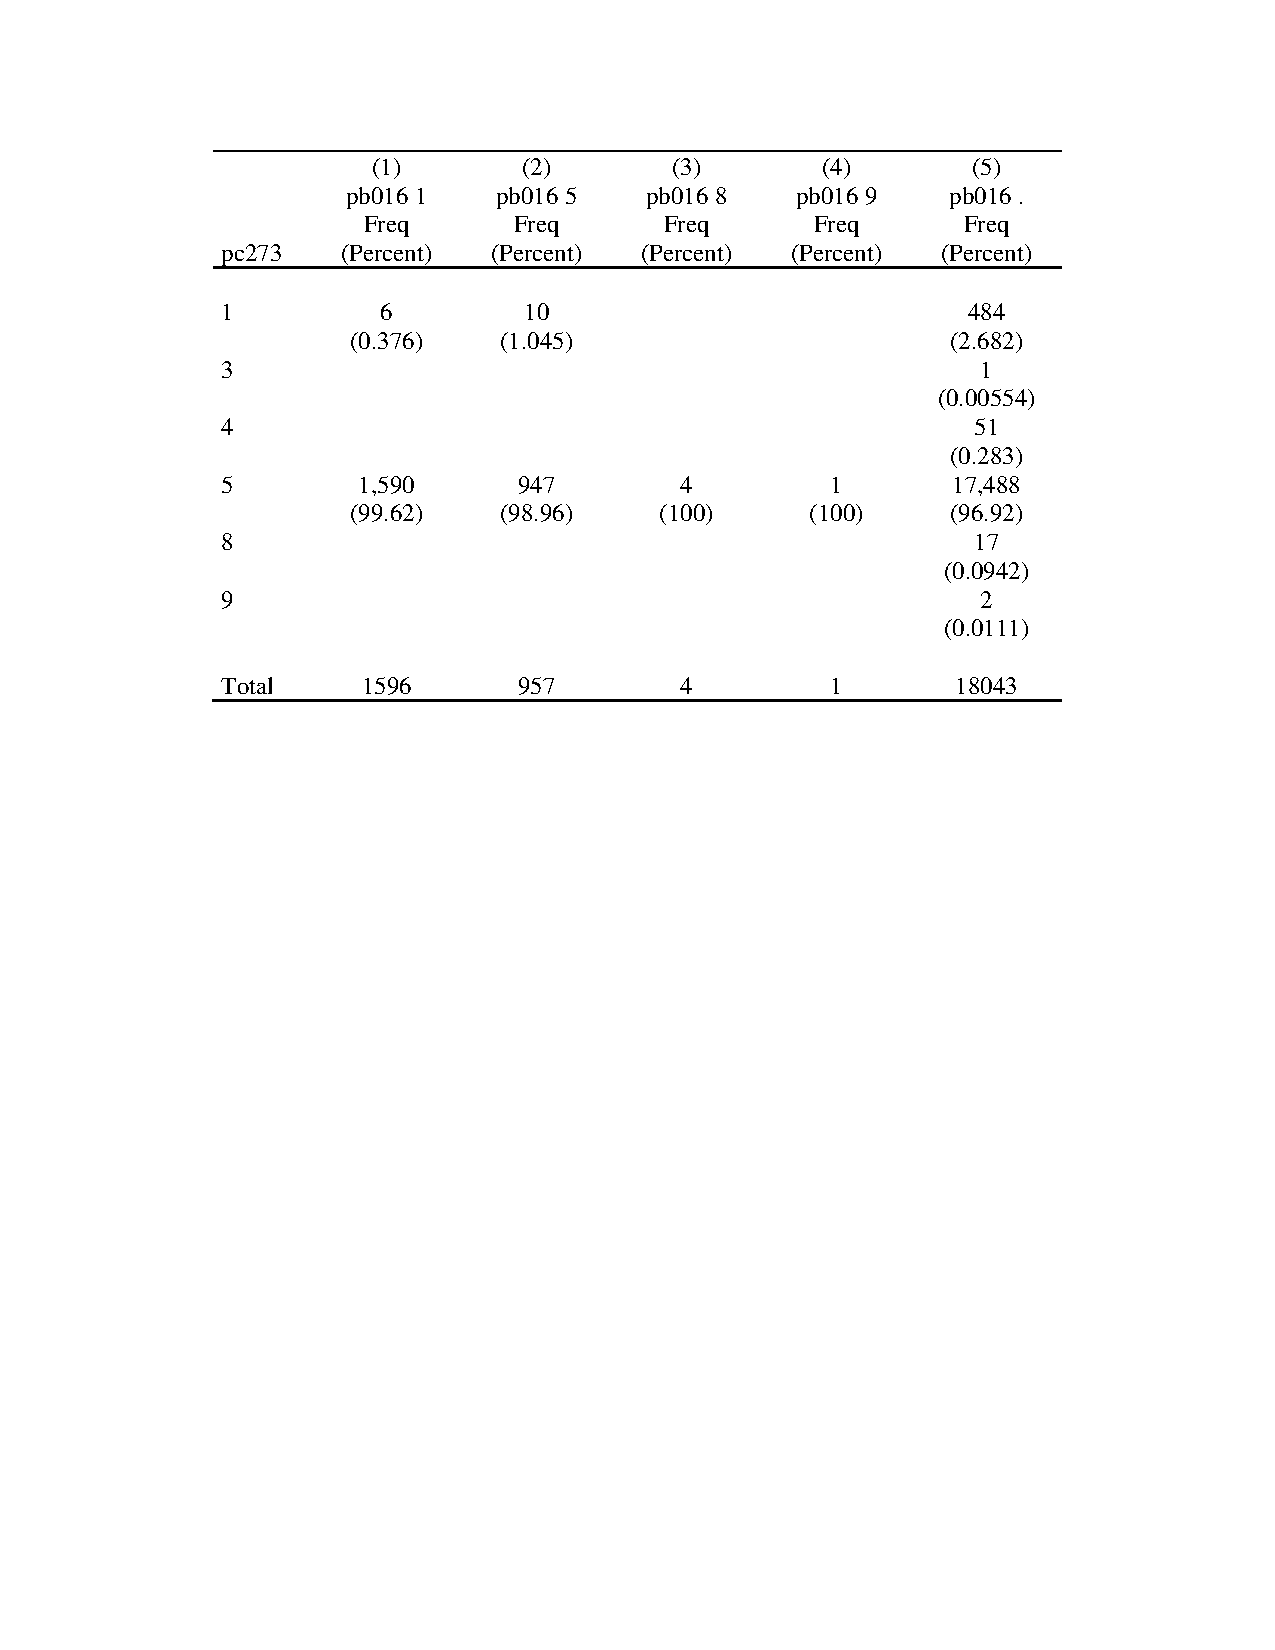
\includegraphics[width=0.5\linewidth]{ever had dementia vs r college degree ctab.doc.pdf}
    \caption{Ever had dementia (PC273) vs college degree (PB016)}
    \label{fig:enter-label}
\end{figure}

\begin{figure}
    \centering
    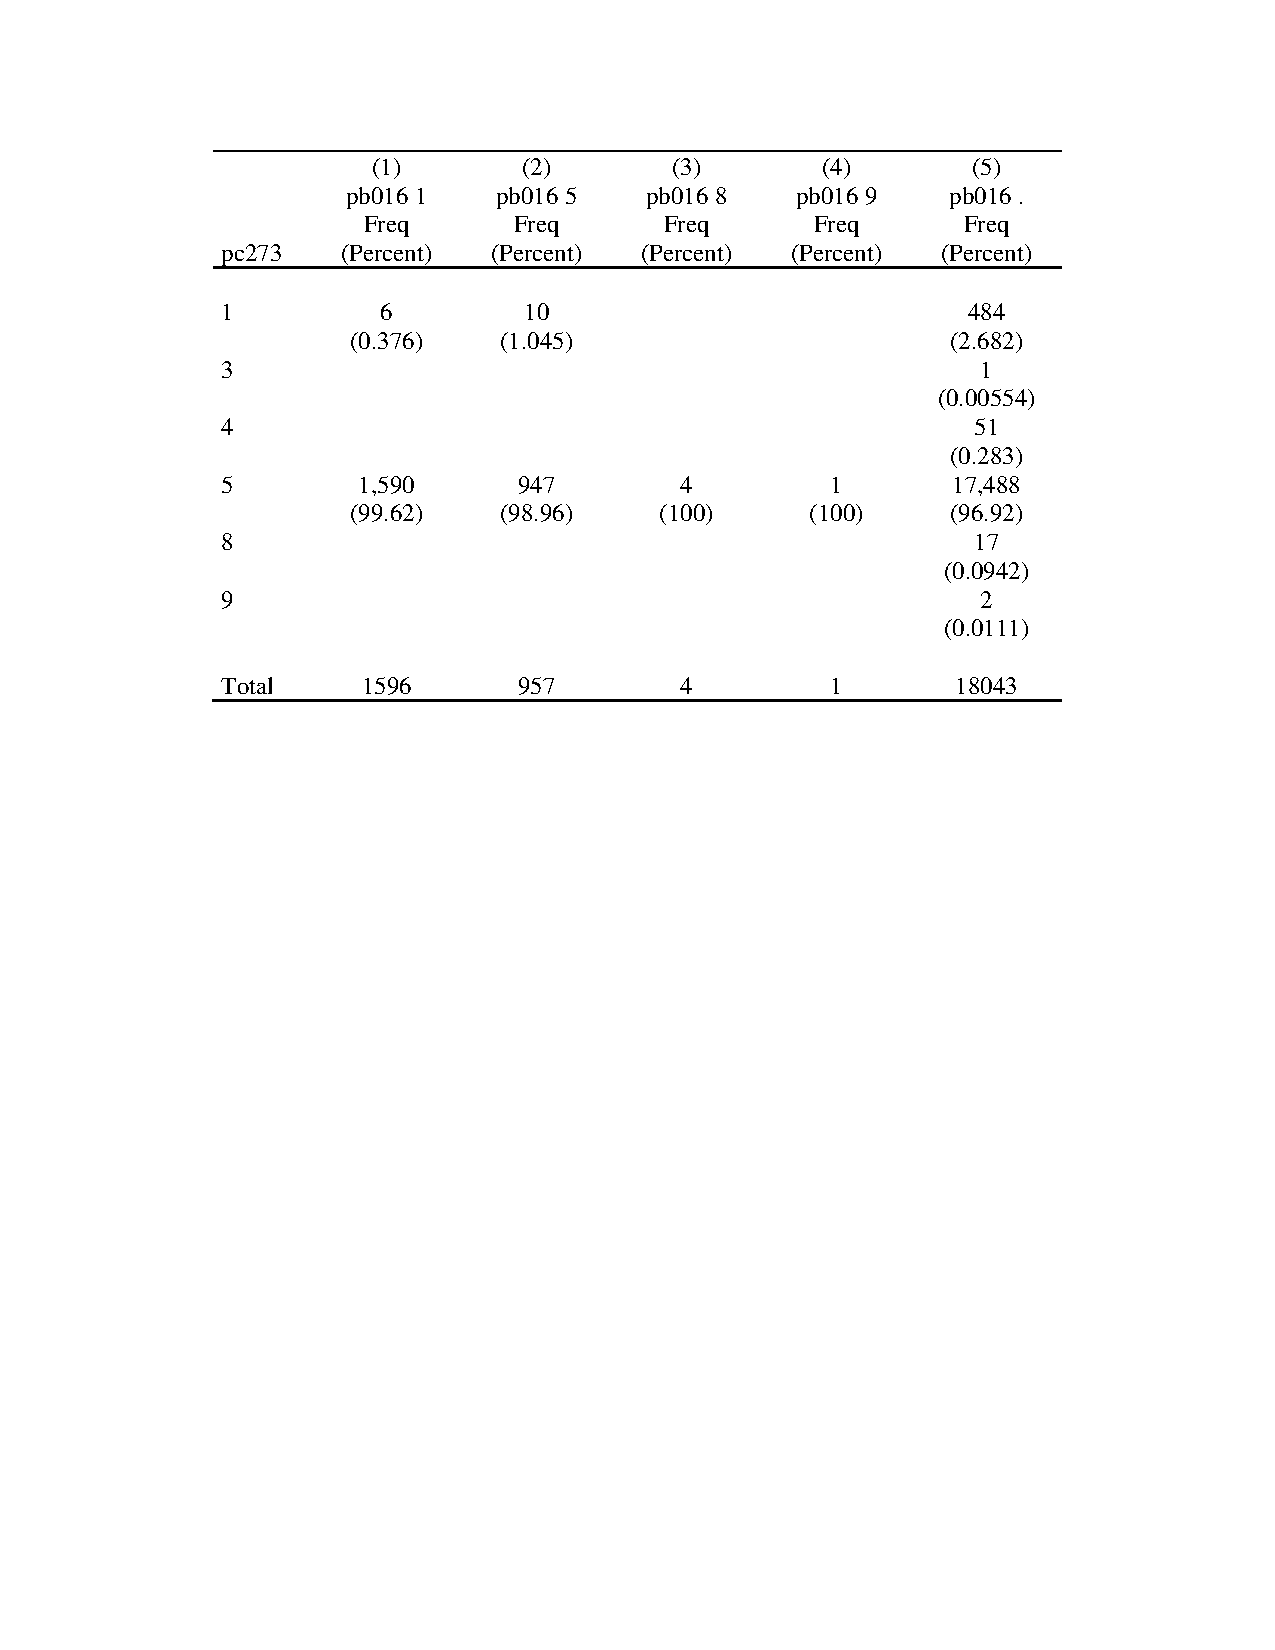
\includegraphics[width=0.5\linewidth]{ever had dementia vs r high school diploma or ged ctab.doc.pdf}
    \caption{Ever had dementia (PC273) vs college degree (PB015)}
    \label{fig:enter-label}
\end{figure}

\begin{figure}
    \centering
    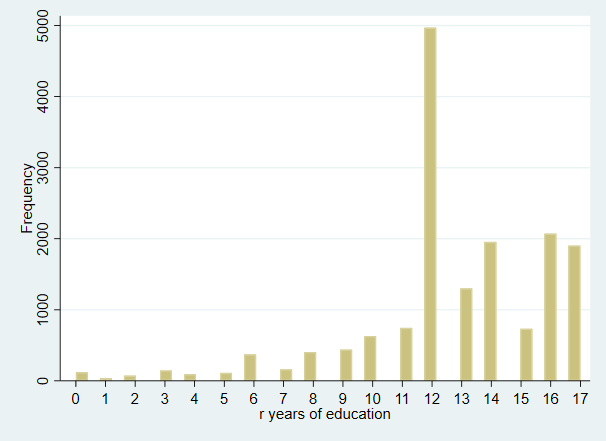
\includegraphics[width=0.5\linewidth]{frequency_histogram_pz216.png}
    \caption{Frequency Histogram of PZ216 (r years of education)}
    \label{fig:enter-label}
\end{figure}

\begin{figure}
    \centering
    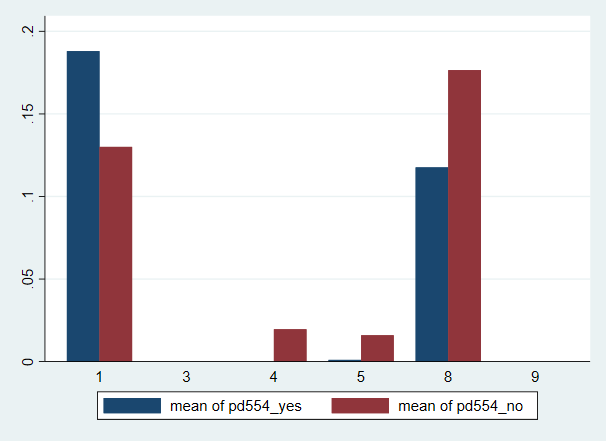
\includegraphics[width=0.5\linewidth]{pd554_over_pc273.png}
    \caption{PD554 (get lost in familiar places) over PC273 (ever had dementia)}
    \label{fig:enter-label}
\end{figure}

\begin{figure}
    \centering
    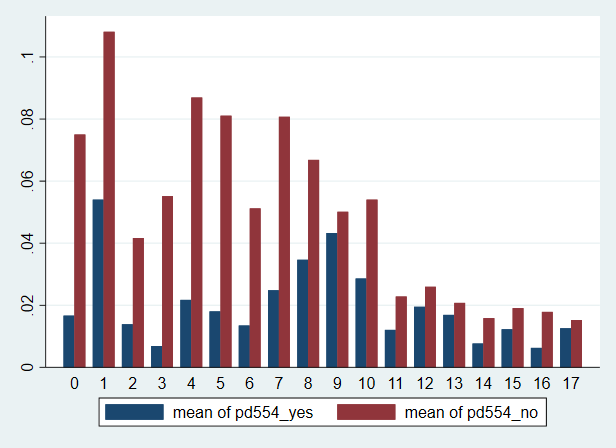
\includegraphics[width=0.5\linewidth]{pd554_over_pz216.png}
    \caption{PD554 (get lost in familiar places) over PZ216 (r years of education)
}
    \label{fig:enter-label}
\end{figure}

\begin{figure}
    \centering
    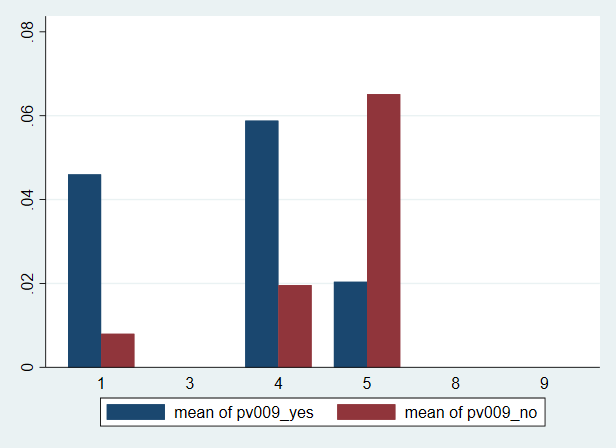
\includegraphics[width=0.5\linewidth]{pv009_over_pc273.png}
    \caption{PV009 (forgetful during daily activities) over PC273 (ever had dementia)}
    \label{fig:enter-label}
\end{figure}

\begin{figure}
    \centering
    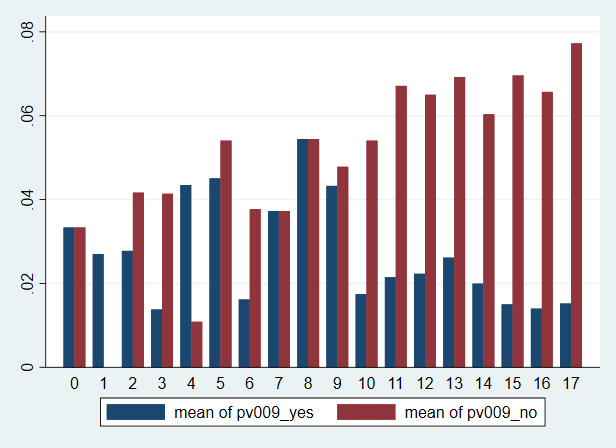
\includegraphics[width=0.5\linewidth]{pv009_over_pz216.png}
    \caption{PV009 forgetful during daily activities) over PZ216 (r years of education)}
    \label{fig:enter-label}
\end{figure}

\begin{figure}
    \centering
    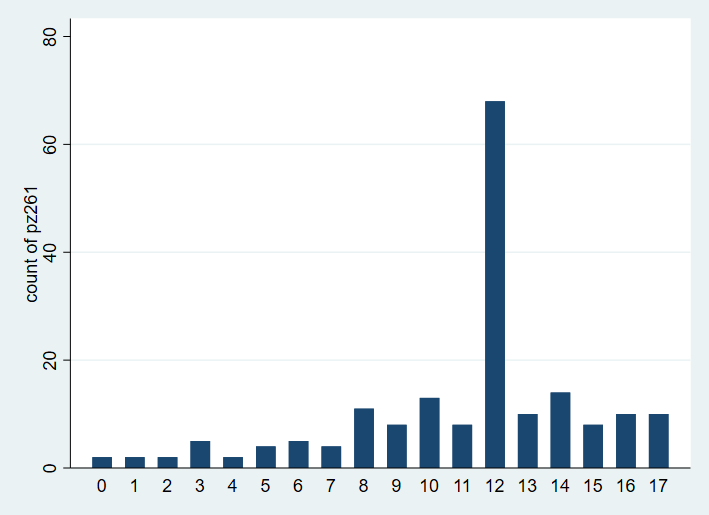
\includegraphics[width=0.5\linewidth]{pz261_over_pz216.png}
    \caption{PZ261 (pw Alzheimer's) over PZ216 (r years of education)
}
    \label{fig:enter-label}
\end{figure}

\begin{figure}
    \centering
    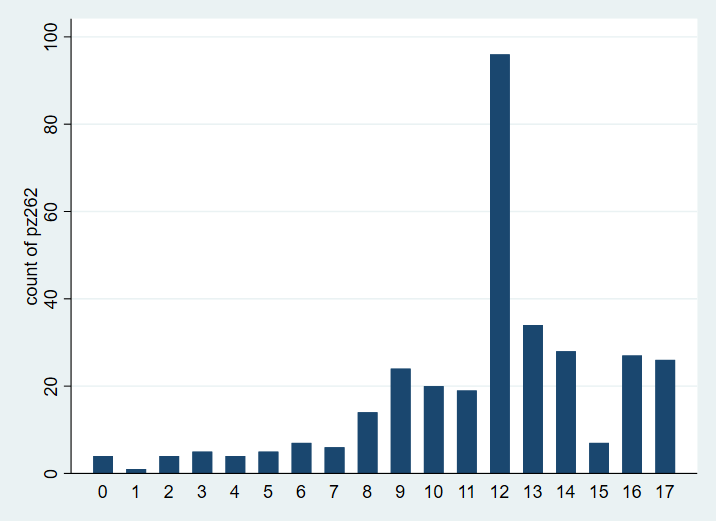
\includegraphics[width=0.5\linewidth]{pz262_over_pz216.png}
    \caption{PZ262 (pw dementia) over PZ216 (r years of education)}
    \label{fig:enter-label}
\end{figure}

\section{Analysis and Results}
\label{sec:result}

\hspace*{1em} We first employed causal diagrams in the early stages of our research to predict the relationships between the variables that were explored during our literature review. We used the articles that we selected when conducting the literature review to frame these diagrams and provide a degree of direction in what we should be looking for in our data. Even though this was made while we were still using the HCAP 2016 dataset, we selected the RAND 2016 dataset based on its similarity to HCAP 2016 and how it just provided more information about our topic. This allowed our causal diagrams to remain relevant. Descriptive statistics was our next mode of exploration and we each selected a different variable from the HCAP 2016 dataset to create bar graphs about. Due to our abandonment of said dataset, the results from this exercise were not helpful. However, we were able to learn how to code for the graphs, their x and y axis titles, exporting to files, and ultimately interpreting our results.

\hspace*{1em} Our hypothesis is exploring the connection between receiving a baseline level of education that eventually improves and strengthens brain function, preventing the development of dementia. We used variables that asked respondents if they have dementia (PC273), if they have Alzheimer’s (PZ261), the years of education they had (PZ216), if they get lost in familiar places (PD554), and are forgetful during daily activities (PV009). These variables were manipulated into a variety of bar graphs that acted as the baseline for our tables that we later created. We also cross tabulated PC273 with PB016, which places if the respondent has ever had dementia and if they ever received a college degree. This was also duplicated but with PB015 replacing PB016, so we could see the frequency of dementia diagnosis with the earning of a high school diploma or GED. There was also an exploration into the respondent’s themselves rating their own memory (PD101).

\hspace*{1em} The graph of PD554 (getting lost in familiar places) over PZ216 (r years of education) shows a weak relationship between those who get lost/don’t get lost and how many years of education they’ve received, due to how the longer bars that correspond with not getting lost in familiar places are towards the lower years of education. When plotting PD554 against PC273 (ever had dementia), we see the higher frequency of those who responded “yes” to getting lost in familiar places are categorized at 1 on the x-axis, which corresponds to responding “yes” to having dementia. The reverse happens at 5, which is where the respondent is saying they don’t have dementia, and more people are also reporting they aren’t getting lost in familiar places. This provides some insight into a possible correlation, but it’s not strong enough to form a definitive conclusion. However, looking at PV009 (forgetful during daily activities) over PZ216 (r years of education) provides stronger evidence of a relationship. There is a clear steady increase in those who responded “no” to being forgetful as their reported years of education increase. This is our main point of reference for our data and resulting inferences. The interpretation of this in conjunction with our hypothesis hints at our projection being correct due to showing that the more time spent in school decreases the likelihood of developing dementia. When PV009 (forgetful during daily activities) was plotted against PC273 (ever had dementia), we can see that those who responded “yes” to being forgetful during daily activities and also having dementia are the larger spike while at 5 on the x-axis (representing someone who doesn’t have dementia), has the largest spike for not being forgetful. Both of these graphs together support our hypothesis even more as they indicate that the increase in years of schooling stimulates brain activity which further increases cognitive health. In the two cross tabulation tables comparing PC273 (ever had dementia) to PB016 (r college degree) and PB015 (r earned high school diploma/GED) we see a stronger relationship in the PB015 table. On both tables, we focused our attention on 1 (yes) and 5 (no) for ever having dementia, and 1 (yes), 5 (no), and 2 (GED) which only shows up on the PC273 versus PB015 table. The difference in frequency between those who have/do not have dementia and whether or not they have a college degree are quite close in value, which does not indicate a strong correlation to us. However, PC273 compared to PB015 provides a clearer picture of our data in relation to our hypothesis. It is evident that the amount of people who earned a high school diploma or GED have a lower frequency of dementia diagnosis. 

    


\section{Discussion}
\label{sec:discussion}

Optional. This is where you would discuss any of the following
\begin{itemize}
    \item caveats (are there problems with the data that there are no obvious ways to resolve? if so, how might this impact
    \item future work / next steps
    \item implications of the results (how your findings -- if they were causally identified -- might inform policymaking, etc.
\end{itemize}

\section{Conclusion}
\label{sec:conclusion}

Re-state (in different words) what you did and what you learned. If your discussion would be short, you can add the discussion after your summary.

\newpage
\section*{Bibliography}
\singlespacing
\setlength\bibsep{0pt}


\newpage
\section*{Appendix A. Placeholder} \label{sec:appendixa}
\addcontentsline{toc}{section}{Appendix A}

\end{document}